% Chapter 5

\chapter{Implementation} % Main chapter title

\label{Chapter5} % For referencing the chapter elsewhere, use \ref{Chapter1} 

%----------------------------------------------------------------------------------------
The designer has evaluated different options to create this software: at the end the option of creating a web application seemed to be the best solution.
Some non-functional requirements, such as the goal to create a solution easily compatible with any machine, without installing nothing, and without creating problems related to the version of Root Framework or the version of gAn, are quite hard to achieve in a stand-alone application. In a web application instead it is easy avoid all the installation and compatibility problems, because it is sufficient solve them only one time on the server, and the user will never has to think about these points. Furthermore, a machine with a windows environment can in this way access to a service executed by a linux system, without problems.  

The only framework used in the interface (Root Framework is used in the back-end) is Bootstrap. Bootstrap is quite useful in the production of the front-end because allows the programmer to manage the dimension of each object on the screen in a smart way and to automatically adapt this dimension to the varying dimension of the screen. It was evaluated the possibility to use a framework for the part related to PHP, but it was preferred not to do so. The point is that the PHP part of the program is quite little and quite atypical: in fact the main task of the PHP part is to talk with the C++ scripts of Root, and for this kind of atypical situation the use of a framework can lead more problems that advantages.  

Everywhere in the program is easily visible the sign of Bootstrap, in particular all the graphical parts are taken from Bootstrap's components (all visible and freely accessible here \url{http://getbootstrap.com/components/}). The goal of this choice is to exploit the wide diffusion of Bootstrap's graphics on the internet: a common user used to navigate on the net surely is used to see the graphical object of Bootstrap, and is unconsciously used to associate these symbols to their signification. So the using on the Bootstrap's graphics can improve the affordance of the interface. 
Bootstrap graphics is an enormous database of object, for this project only a few are used, in particular:

\begin{enumerate}

\item The buttons

\begin{figure}[H]
\centering
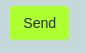
\includegraphics[scale=0.5]{BootstrapButton.png} 
\caption{A button created with Bootstrap's graphics}
\end{figure}

\item The navbar:
This object allow to select a button by clicking on it: when the button is selected the graphical effect changes automatically the color, that became more dark, and give the graphical impression of the button physically pushed, making the user aware of what is the selected button. 

\begin{figure}[H]
\centering
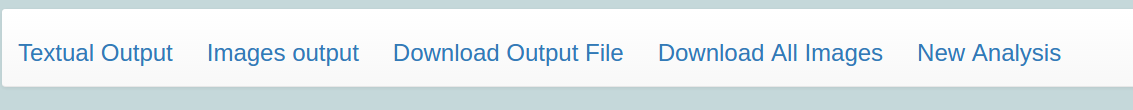
\includegraphics[scale=0.35]{BootstrapNavbar.png} 
\caption{A navbar containing some buttons created with Bootstrap's graphics}
\end{figure}

\item The progress bar

\begin{figure}[H]
\centering

\includegraphics[scale=0.35]{BootstrapProgressBar.png} 
\caption{An infinite ProgressBar created using Bootstrap's graphics}
\end{figure}

This solution makes the waiting time less frustrating for the user. The bar is infinite (without a percentage, it go on like an endless screw until the program is ready to show the results), because it is impossible to estimate precisely the amount of time that the user must wait.

\item The input fields

\begin{figure}[H]
\centering
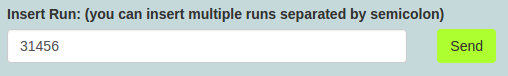
\includegraphics[scale=0.5]{BootstrapInputField.png} 
\caption{An example of input field taken from Bootstrap's graphics}
\end{figure}

\item The dropdown menus

\begin{figure}[H]
\centering
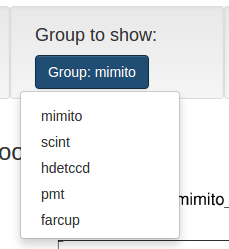
\includegraphics[scale=0.5]{BootstrapDropdownMenu.png} 
\caption{A dropdown menu created with Bootstrap's graphics}
\end{figure}

It is the common solution to force the users to choice a value among some options. According to the users it is aesthetically better than the radio buttons.

\item The tooltips

\begin{figure}[H]
\centering
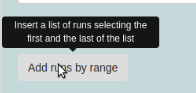
\includegraphics[scale=0.5]{BootstrapTooltip.png} 
\caption{An explaining tooltip obtained form Bootstrap's graphics}
\end{figure}

The user can see this kind of tip just moving the mouse over the interested object. The tip explain briefly what the object can do.

\item The modal form

\begin{figure}[H]
\centering
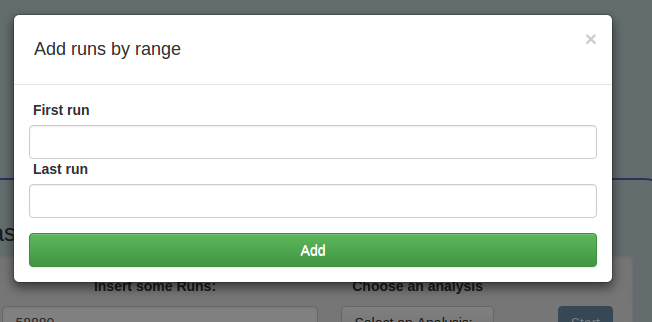
\includegraphics[scale=0.5]{BootstrapModal.png} 
\caption{A modal form obtained form Bootstrap's graphics}
\end{figure}

This structure, named "modal form", is a window that appears on the screen as response to some event, takes the focus, and allow the user to execute some activities. 

\end{enumerate}

\section{TODO}
